\section{Algebrotopologiset määritelmät}

Tässä työssä solmujen ominaisuuksien tutkimiseen tarvitaan topologisia työkaluja. Tämän osion päätarkoituksena on määritellä harvinaisia, solmuteorialle tyypillisiä konstruktioita ja peruskäsitteistö oletetaan lukijan hallitsemaksi.\footnote{Topologian peruskäsitteistöä tuntematonta lukijaa suositetaan perehtymään esimerkiksi tiiviiseen luentomuistiinpanoon \citep{koski2024topology} tai syvällisempään johdantoon \citep{Munkres2000}.} Algebrallisen topologian käsitteistössä seuraillaan Hatcherin \citep{Hatcher2002} kirjaa.

Tämä osio palvelee kahta tarkoitusta: putkiympäristön käsitteen kehittämistä sekä teknisempää todistusta siitä, että kahden homologisen $n$-pallon yhteen pujominen\footnote{Pujominen määritellään solmuja koskevassa kappaleessa ???} tuottaa homologisen $n$-pallon. Käyrän putkiympäristöä voi ajatella pienenä käyrää seurailevana täytettynä putkena. Homologisia palloja koskeva lause varmistaa, että kun kaksi eri avaruuksissa elävää solmua pujotaan yhteen, elää tulossolmu myös ``hyvänlaatuisessa'' avaruudessa.

Formaaleista muotoiluista kiinnostunut lukija voi tutustua osakappaleisiin tarkemmin, mutta niiden sivuuttaminen ei estä lainkaan myöhempiin kappaleisiin perehtymistä.

\subsection{Kimput}
Kuitukimppua voidaan pitää topologisten avaruuksien tulon $X\times Y$ yleistyksenä sikäli, että se sallii ``vääntyneen'' tulon. Vektorikimppu on kuitukimpun erityistapaus.
\begin{maaritelma}[Kuitukimppu]
    \emph{Kuitukimppu} on nelikko $(E,B,\pi,F)$, missä $E,B$ ja $F$ ovat topologisia avaruuksia ja $\pi:E\to B$ jatkuva surjektio, joka tyydyttää paikallisen triviaaliuden ehdon (alla). Sivu 386 alg. top. kirjasta.
\end{maaritelma}
\begin{huomautus}
    Jos $E$ on muotoa $A\times B$, puhutaan ``triviaalista $A$-kimpusta yli $B$:n''.
\end{huomautus}
Kuitukimpun pitää olla paikallisesti triviaali eli muistuttaa tavallista tuloa, mutta globaalisti sen geometria voi olla vääntynyt. Kuva~\ref{kuva:mobius-nauha} esittää epätriviaalisti vääntynyttä sylinteriä $\S^1\times I$, missä $I\subset\R$, eli Möbius-nauhaa.
\begin{figure}
    \centering
    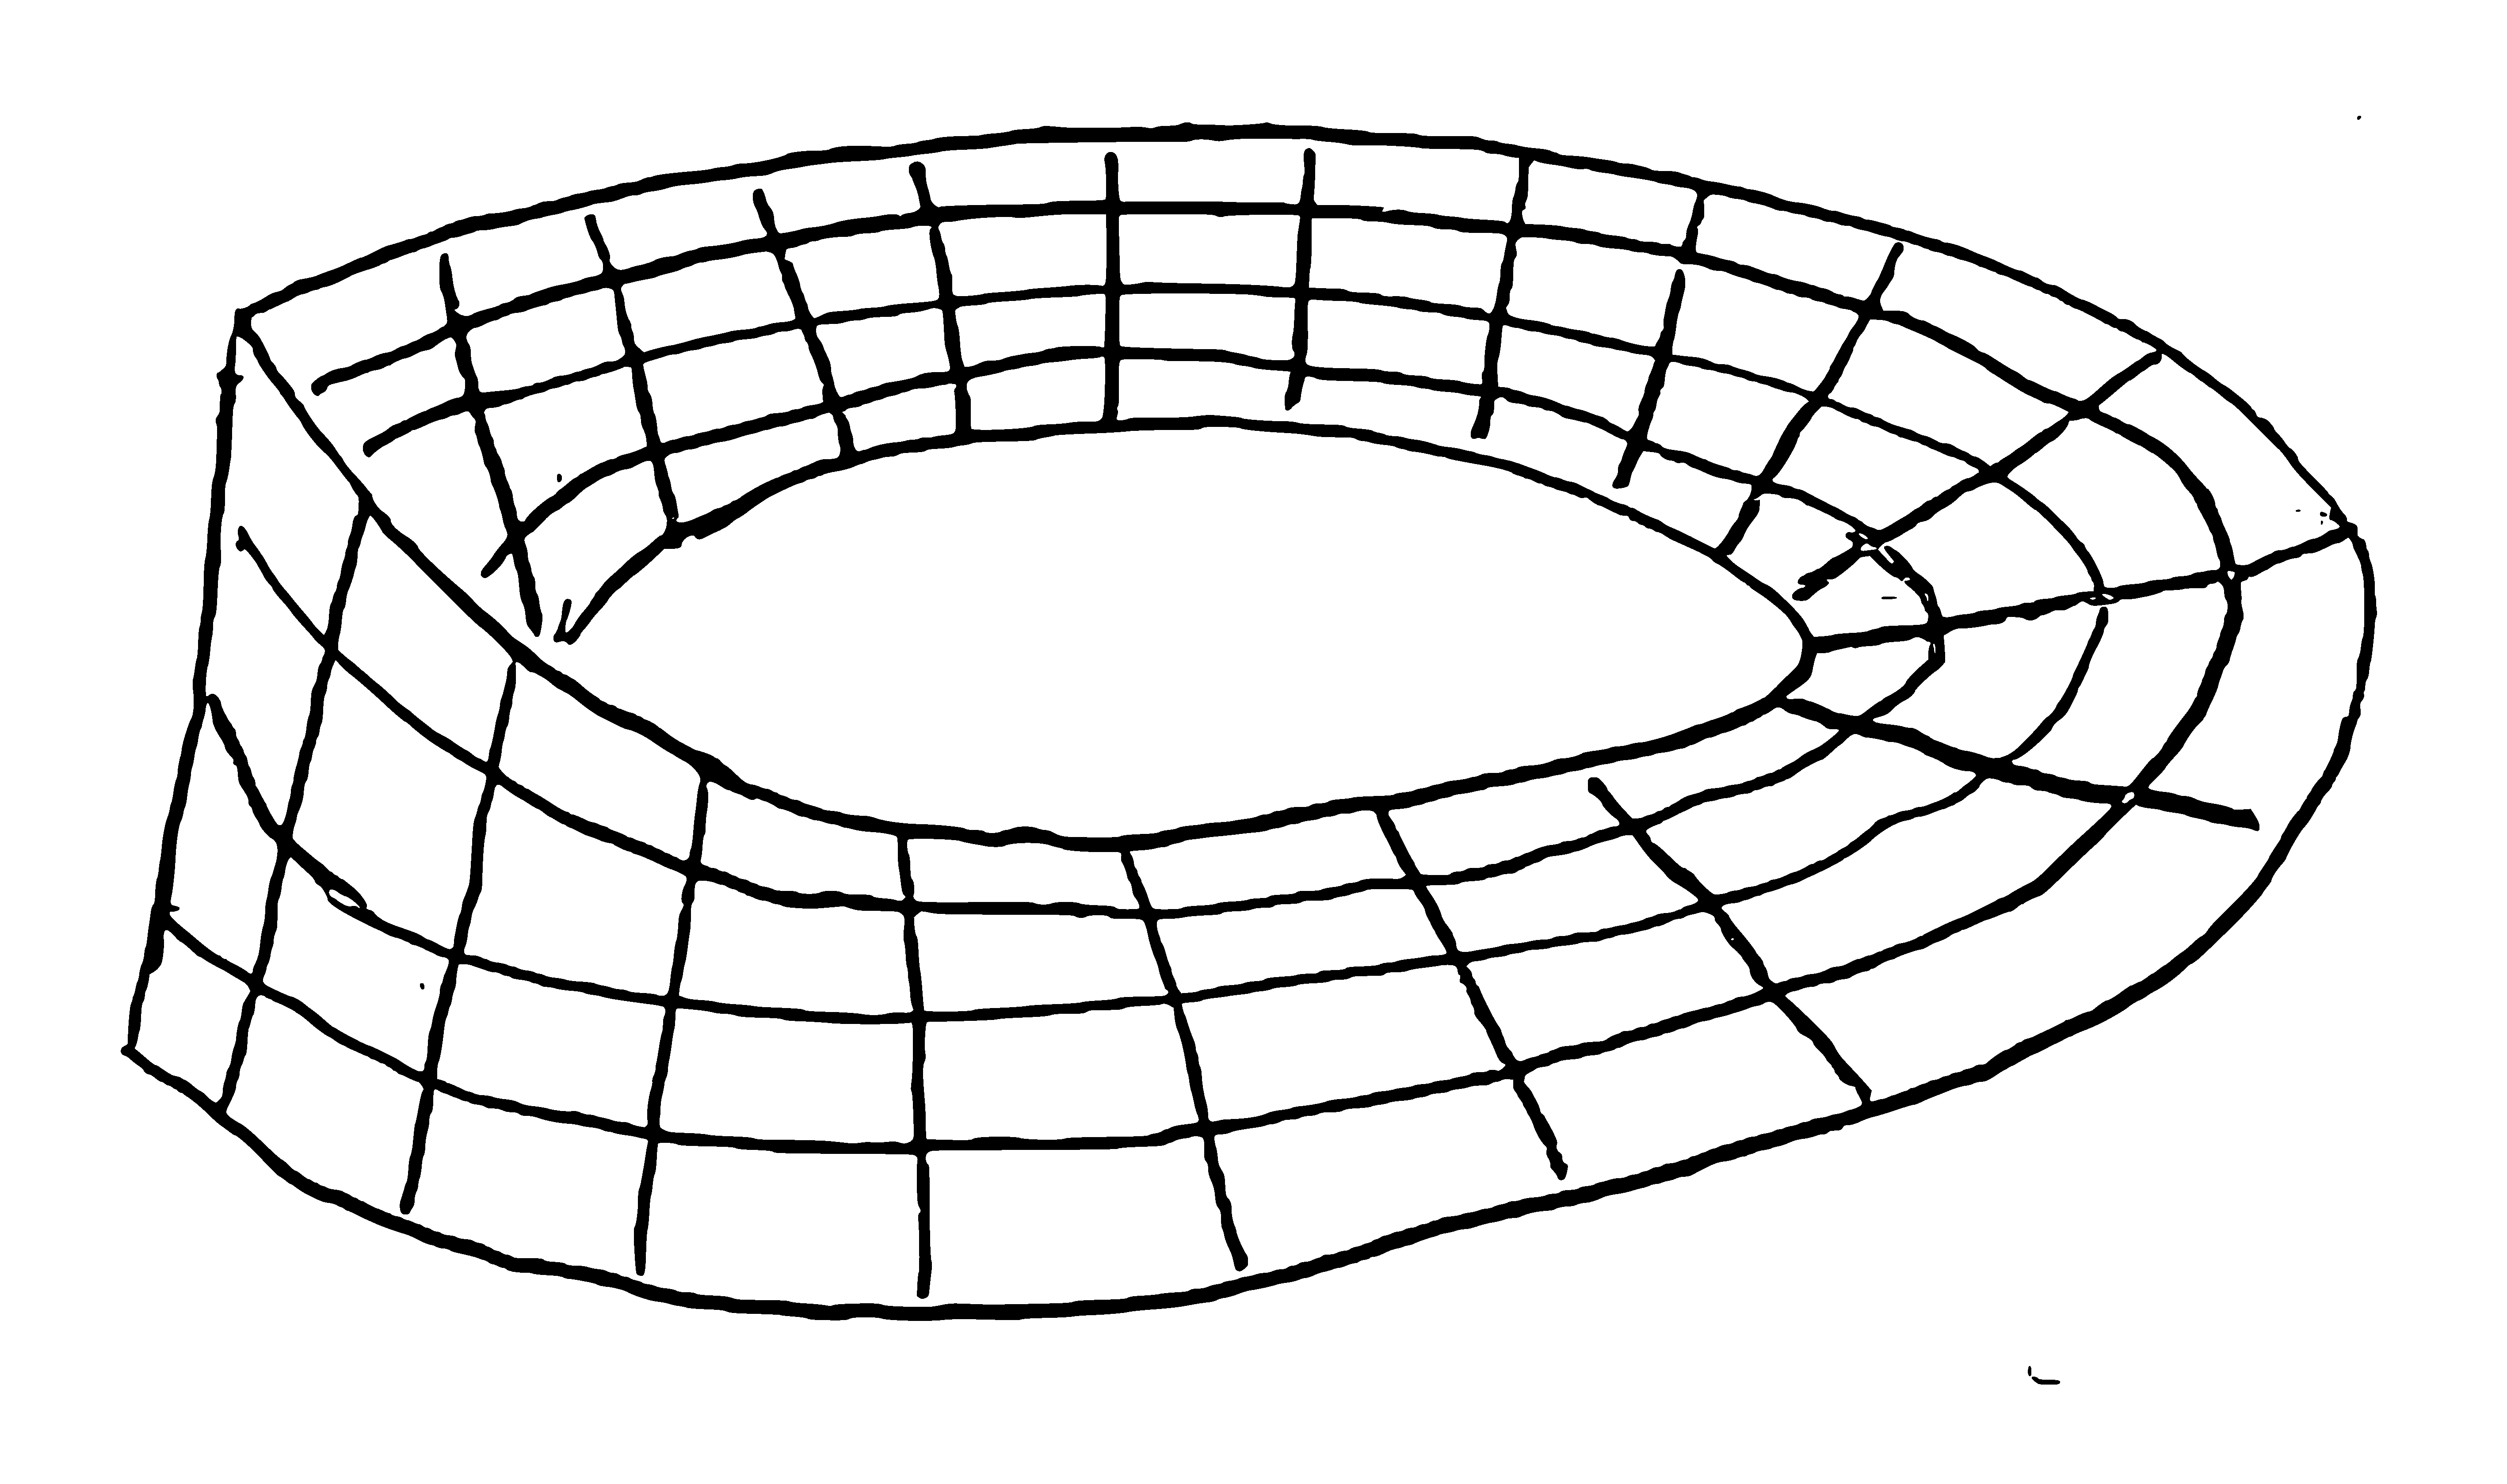
\includegraphics[width=0.5\textwidth]{figures/mobius-nauha.pdf}
    \caption{Möbius-nauha.}
    \label{kuva:mobius-nauha}
\end{figure}
\begin{maaritelma}[Vektorikimppu]
    Olkoon $M$ topologinen avaruus. Asteen $k$ $\K$-\emph{vektorikimppu} $M$:n yli on jatkuvalla surjektiolla $\pi:E\to M$ varustettu topologinen avaruus $E$ siten, että 
    \begin{enumerate}
        \item kaikille $p\in M$ kuitu $E_p=\pi^{-1}(p)$ yli $p$:n voidaan varustaa $k$-ulotteisen $\K$-vektoriavaruuden rakenteella ja
        \item kaikille $p\in M$ on olemassa $p$:n ympäristö $U\subset M$ ja homeomorfismi $\Phi:\pi^{-1}(U)\to U\times\K^k$ siten, että
        \begin{itemize}
            \item $\pi_U\circ\Phi=\pi$ (jossa $\pi_U:U\times\K^k\to U$ on projektio) ja
            \item kaikille $q\in U$ $\Phi|_{E_q}$ on vektoriavaruusisomorfia $E_q\cong\{q\}\times\K^k\cong\K^k$.
        \end{itemize}
    \end{enumerate}
\end{maaritelma}
\begin{esimerkki}
    Esimerkiksi pallo ja sen tangenttikimppu muodostavat vektorikimpun $\pi:T\S^2\to\S^2$, jossa projektio määritetään $T_p\S^2\mapsto p$ eli pisteeseen, jossa tangenttiavaruus kiinnittyy palloon. Tässä jokainen kuitu voidaan varustaa 2-ulotteisella $\R$-rakenteella.
\end{esimerkki}
Pallo ja tangenttikimppu ovat esimerkkejä globaalisti triviaalista vektorikimpusta, jossa ei ole vääntöä. Yleisemmässä vektorikimppujen tapauksessa puhutaan tangenttiavaruuksien sijaan tangenttikuidusta, jossa voi olla globaalia vääntöä.


\subsection{Kuidut}
Siinä missä kuitukimppu yleistää topologisen tulon, kuidutus yleistää kuitukimpun. Kuidutuskonstruktio on hankala käsittää ja se esitetään tässä pääosin vain myöhempää konstruktiota, putkiympäristöä, varten.
\begin{maaritelma}[Homotopinen nosto-ominaisuus]
    Kuvaus $\pi:E\to B$ tyydyttää \emph{homotopisen nosto-ominaisuuden} avaruudelle $X$, jos
    \begin{itemize}
        \item kaikille homotopioille $g:X\times[0,1]\to B$ ja
        \item kaikille kuvauksille $\tilde g_0:X\to E$ nostaen $g_0=g(\cdot,0)$:n, eli $p\circ\tilde g_0=g_0$,
    \end{itemize}
    on olemassa homotopia $\tilde g:X\times[0,1]\to E$ nostaen $g$:n (eli $g=p\circ\tilde g$) niin, että $\tilde g_0=\tilde g|_{X\times\{0\}}$. Kommutoiva kaavio havainnollistaa tilanteen:
    \begin{equation}
        \begin{tikzcd}
            X\times\{0\} \arrow[r, "\tilde g_0"] \arrow[d, hook] & E \arrow[d, "\pi"] \\
            X\times[0,1] \arrow[ur, dashrightarrow, "\tilde g"] \arrow[r, "g"] & B
        \end{tikzcd}
    \end{equation}
\end{maaritelma}
\begin{maaritelma}
    \emph{Kuidutus} on kuvaus $\pi:E\to B$, jolla on homotopinen nosto-ominaisuus kaikkien avaruuksien $X$ suhteen.
\end{maaritelma}
\begin{maaritelma}
    Olkoon $\pi:E\to B$ kuidutus. Kuidutus on \emph{paikallisesti triviaali}, jos kaikille $x\in B$ on olemassa avoin ympäristö $U\subset B$ ja $F\subset E$ siten, että 
    \begin{equation*}
        \pi^{-1}(U)\approx U\times F.
    \end{equation*}
\end{maaritelma}
\begin{maaritelma}
    Jos $E$ on pohja-avaruuden $B$ kuitukimppu $\pi:E\to B$, niin \emph{kuitukimpun sektio} on jatkuva kuvaus $\sigma:B\to E$ siten, että $\pi\circ\sigma=\text{id}_B$.
\end{maaritelma}

\subsection{Putket}
\begin{maaritelma}
    Olkoot $S,M$: $S\subset M$ sileitä monistoja. $S$:n \emph{putkiympäristö} $M$:ssä on pari $(\pi, J)$, jossa $\pi: E\to S$ on vektorikimppu ja $J:E\to M$ on sileä kuvaus, siten että
    \begin{itemize}
        \item $J\circ0_E=i$, $i$ on upotus $S\hookrightarrow M$ ja $0_E$ nollasektio
        \item on olemassa avoimet joukot $U\subset E$, $V\subset M$ siten, että $0_E[S]\subset U$ ja $S\subset V$ niin, että rajoitus $J|_U$ on diffeomorfismi.
    \end{itemize}
\end{maaritelma}
Yksinkertainen esimerkki saadaan käyrästä $\R^3$:ssa. Sen putkiympäristö on käyrää seuraileva kolmiulotteinen mato, jonka poikkileikkaukset ovat tasojoukkoja, joiden muoto vaihtelee, mutta käyrän suuntaisesti aina sileästi. Käyrän putkiympäristön läpileikkaus ei välttämättä ole täydellinen ympyrälevy keskusakselin (käyrän) ympäri, mutta topologisesti se on aina ympyrälevy. Esimerkki kuvassa~\ref{kuva:putkiympäristö}.
\begin{figure}
    \centering
    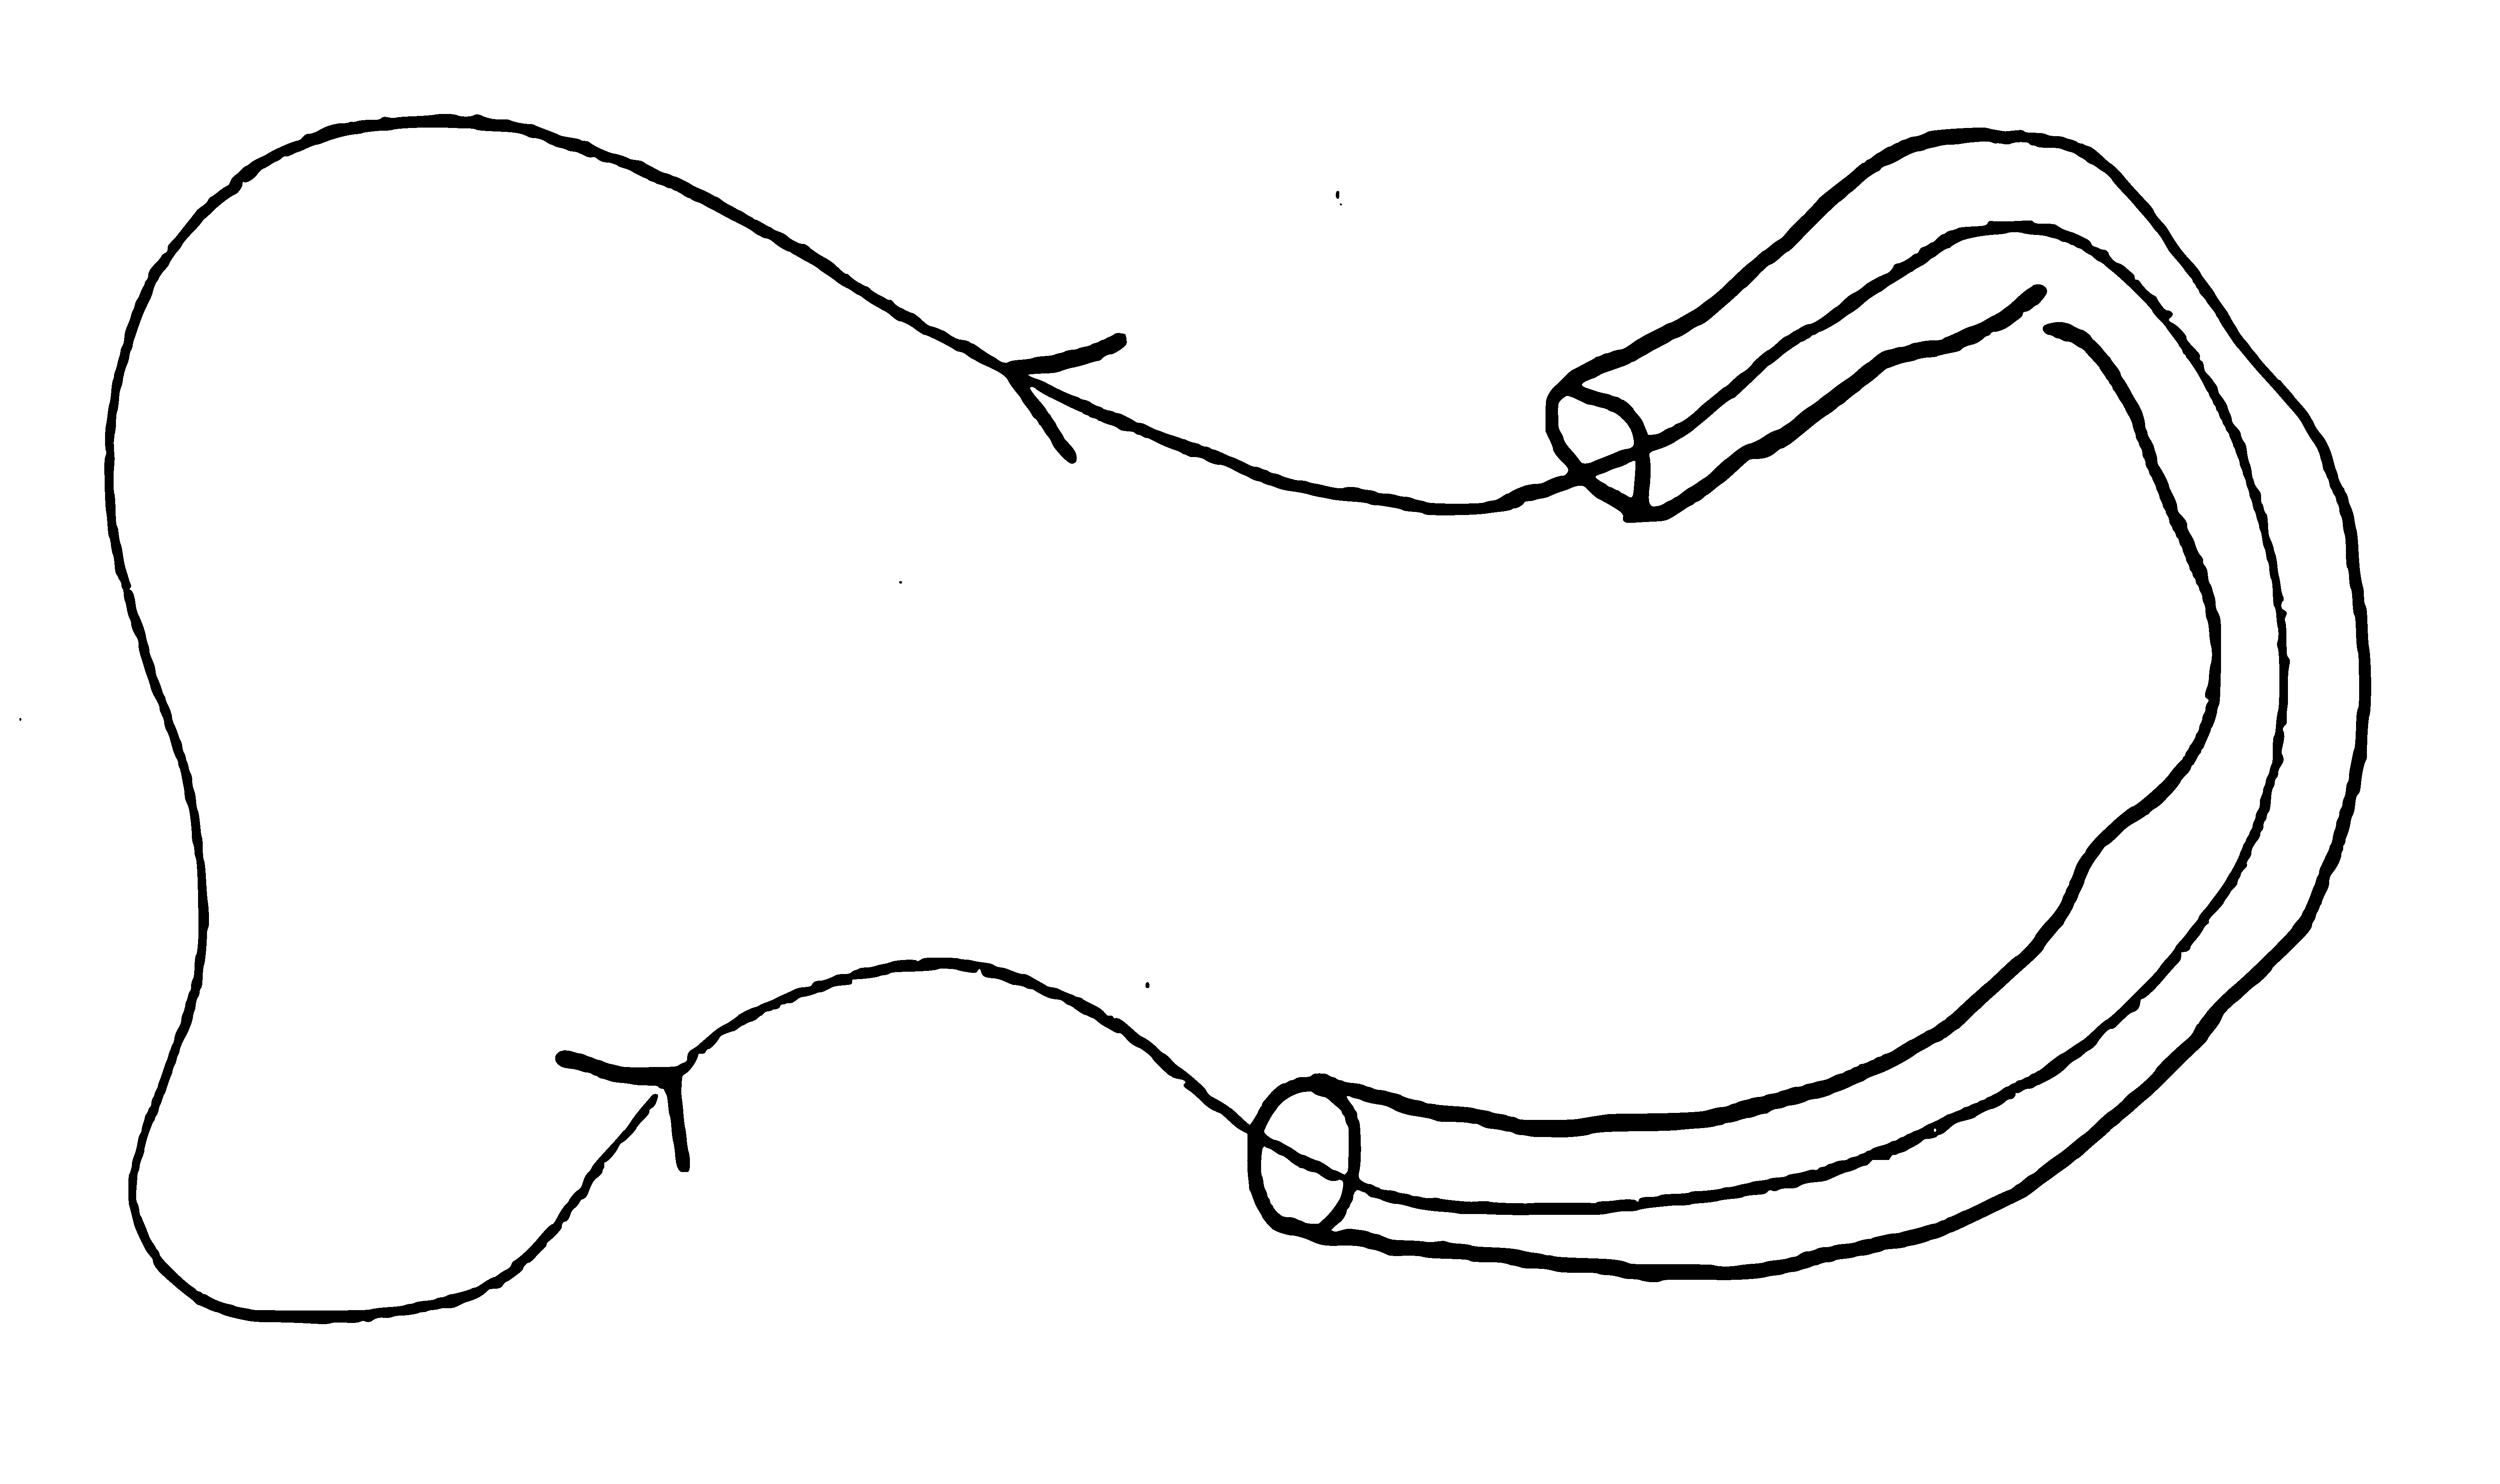
\includegraphics[width=0.5\textwidth]{figures/putkiympäristö.pdf}
    \caption{3-monistoon upotettu suljettu käyrä, jolle piirretty pätkä mielivaltaista putkiympäristöä.}
    \label{kuva:putkiympäristö}
\end{figure}
\begin{lause}[Putkiympäristölause]
    Jokaisella sileän moniston upotetulla sileällä alimonistolla on putkiympäristö.
\end{lause}
\begin{proof}
    Todistus on vaikea ja löytyy lähteestä ???.
\end{proof}
\begin{maaritelma}
    Olkoon $f:\C^2\to\C$ polynomikuvaus. Sen kuitua $f^{-1}(c),c\in\C$ kutsutaan \emph{säännölliseksi}, mikäli jollekin $c$:n ympärisölle $D$ kuvaus $f|_{f^{-1}(D)}:f^{-1}(D)\to D$ on paikallisesti triviaali $C^\infty$-kuidutus.

    Kuitu $f^{-1}(c)$ on \emph{säännöllinen äärettömyydessä}, jos jollekin $c$:n ympäristölle $E$ ja kompaktille osajoukolle $K\subset\C^2$ kuvaus $f|_{f^{-1}(D)-K}$ on paikallisesti triviaali kuidutus. 

    Jos kaikki $f$:n kuidut ovat säännöllisiä äärettömyydessä niin $f$ on \emph{hyvä}.
\end{maaritelma}
\begin{huomautus}
    ``Säännöllinen'' ja ``säännöllinen äärettömyydessä ja epäsingulaarinen'' ovat yhtäpitäviä.
\end{huomautus}
\begin{ajatus}
    Säännöllisyys on matemaattinen muotoilu idealle, että läheiset kuidut ``näyttävät samalta'' kuin $f^{-1}(c)$. Säännöllisyys äärettömyydessä muotoilee tämän samalta näyttämisen äärettömyyden ``lähellä''.
\end{ajatus}

\subsection{Homologiaa pintapuolisesti}
Homologia on sisällöltään runsas ja tekninen matematiikan osa-alue, jonka tarkoituksena on tutkia topologisten avaruuksien rakennetta ja reikiä. Homologian ehtisi tässä työssä esitellä vain lyhyesti, mikä ei tee aihepiirille oikeutta syvyytensä vuoksi; siispä aiheen esittely ohitetaan tässä työssä, mutta kiinnostunutta lukijaa ohjataan tutustumaan erinomaiseen Hatcherin materiaaliin \citep{Hatcher2002}. Tässä tarkastellaan vain soluhomologiaa, hieman yksinkertaistettua homologian teoriaa.

Tässä aliosiossa esitetään kuitenkin lyhyt motivaatio homologialle sekä määritellään pari työssä keskeistä käsitettä. Määritelmät tarjoillaan intuitivistisen selityksen kera, homologiaa tuntematonta lukijaa silmälläpitäen.
\begin{ajatus}
    Homologia tutkii topologisten avaruuksien \emph{erilaisuutta} avaruuksien \emph{reikäisyyden} kautta. Reikäisyys on yllättävän vaikeaa määritellä, mutta se auttaa myös yllättävän hyvin erottelemaan avaruuksia toisistaan, esimerkiksi pallon ja toruksen.
\end{ajatus}
\begin{esimerkki}
    Ympyrä $\S^1$ ja kahdeksikko eivät ole homologisia. Ympyrä sulkee sisäänsä yhden reiän, kahdeksikko kaksi reikää.
\end{esimerkki}
Ympyrän sulkema reikä on olemassa, koska ympyrä muodostaa silmukan. On tärkeää huomata, että silmukka on yksiulotteinen. Korkeamman asteen reiän sulkee sisäänsä $\S^2$, joka on kaksiulotteinen. Tämäkin on tosiaan reikä; siihen ei voi päästä kolmiulotteisessa avaruudessa käsiksi kulkematta $\S^2$:n pinnan läpi, mutta neljättä ulottuvuutta pitkin reiän läpi voi kulkea koskematta $\S^2$:een.

Käytännössä homologiassa lasketaan homologiaryhmiä $H_n(X)$, missä $X$ on topologinen avaruus. Alaindeksi $n\in\Z$ kertoo, että kyseessä on $n$:s homologiaryhmä, joka tavallaan mittaa avaruuden $n$-ulotteisia reikiä. Muitakin kuin kokonaislukukertoimia voisi käyttää, mutta tässä työssä rajoitutaan selkeyden vuoksi kokonaislukukertoimiin.
\begin{esimerkki}
    Ympyrälle $\S^1$ homologiaryhmät ovat
    \begin{equation*}
        H_i(\S^1)=
        \begin{cases}
            \Z, & i=0,1 \\
            0, & i>1
        \end{cases}.
    \end{equation*}
    Nollas homologiaryhmä $H_0$ mittaa avaruuden yhtenäisten komponenttien määrää. $H_0(\S^1)=\Z$ tarkoittaa, että ympyröitä voisi olla $k$ kappaletta liimattuna päällekkäin, $k\in\Z$ tai nolla, jos $k=0$.

    $H_1$ mittaa 1-ulotteisten silmukoiden muodostamien reikien määrää.

    $H_n$ mittaa $n$-ulotteisten ``silmukoiden'' jättämien reikien määrää, mutta $\S^1$:llä ei ole $n$-ulotteisia silmukoita.
\end{esimerkki}
\begin{esimerkki}
    Pallon $\S^2$ tapauksessa $H_2(\S^2)=\Z$, mutta $H_1(\S^2)=0$, koska pallon pinnalle piirretyn ympyrän voi aina kiristää pisteeksi, mutta pinnan sisäänsä sulkevaa huppua ei voi.
\end{esimerkki}
Mitä ympyröiden homologiaryhmiin tulee, lukija saattoi huomata jo kaavan, joka todistetaan lemmassa~\ref{lemma:ympyröiden-homologia}.
\begin{lemma}
    \label{lemma:ympyröiden-homologia}
    Kaikille $n$-palloille $\S^n$ pätee
    \begin{align*}
        H_0(\S^n)&=H_n(\S^n)=\Z, \\
        H_k(\S^n)&=0,\quad k\ne n.
    \end{align*}
\end{lemma}
\begin{proof}
    Todistus perustuu \emph{Mayer-Vietoris-jonoon}, joka on hieman edistynyt homologian konstruktio. Tiiviyden vuoksi todistus sivuutetaan, mitä puoltaa se, että tulos on yleisesti tunnettu ja hyväksytty.
\end{proof}
Kenties tärkein homologian sovellutus tässä työssä on vielä esittelemättä. Vilkaistaan toruksen homologiaryhmiä.
\begin{esimerkki}
    Toruksella $\T^2=\S^1\times\S^1$ on mielenkiintoisempia ryhmiä:
    \begin{equation*}
        H_i(\T^2)=
        \begin{cases}
            \Z, & i=0,2 \\
            \Z\oplus\Z, & i=1 \\
            0, & i>2
        \end{cases}
    \end{equation*}
    Ryhmä $H_1$ selittyy sillä, että toruksen pinnalle voi piirtää kaksi silmukkaa, joita ei voida muuntaa toisikseen: toruksen ison akselin ympäri, sekä toruksen paksuutta pitkin. Tämä on havainnollistettu kuvassa~\ref{kuva:toruksen-homologia-akselit}
\end{esimerkki}
\begin{figure}
    \centering
    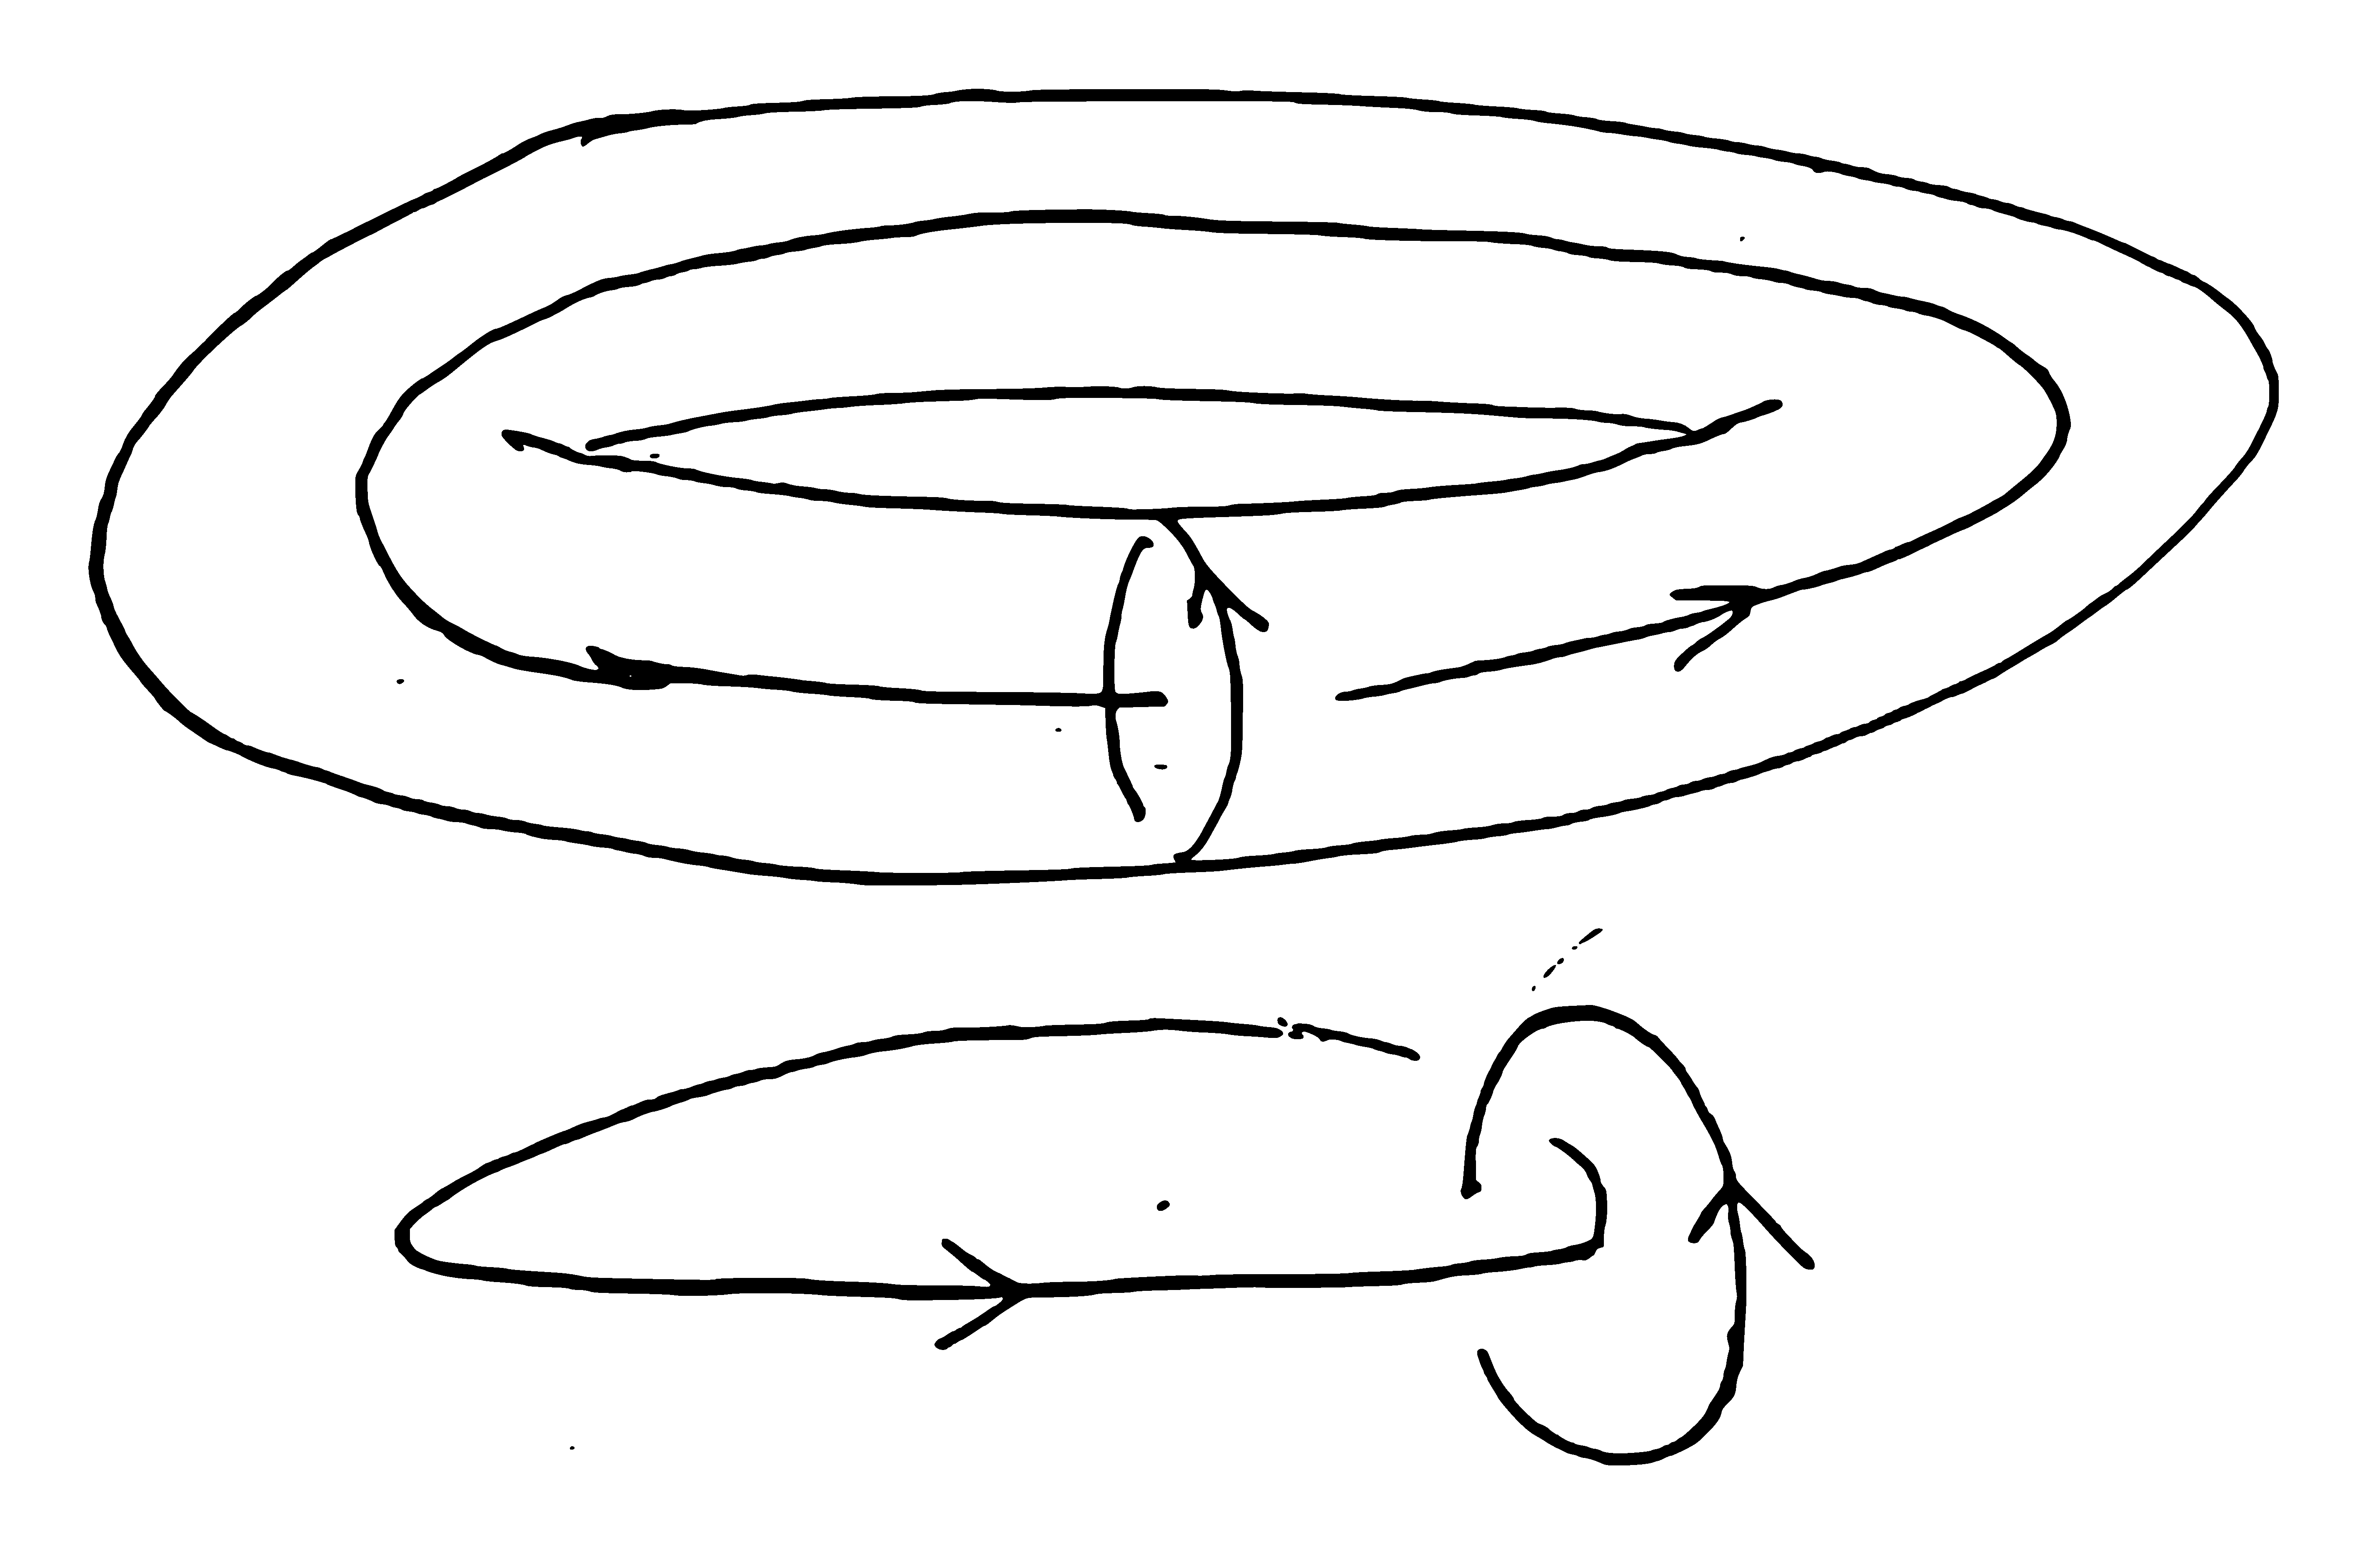
\includegraphics[width=0.5\textwidth]{figures/toruksen-homologia-akselit.pdf}
    \caption{Toruksen kaksi homologia-akselia.}
    \label{kuva:toruksen-homologia-akselit}
\end{figure}
Jos $\solmu\subset\T^2$ on toruksen pinnalla kulkeva suljettu, itseään leikkaamaton, suunnattu käyrä niin sen voi kuvata yksiselitteisesti toruksen homologia-akseleiden avulla. Tällaiset käyrät ovat tärkeä konstruktio tässä työssä, joten seuraava määritelmä on mielekäs.
\begin{maaritelma}
    Olkoon $\TT^2=\S^1\times \D^2$ täytetty torus. Olkoot $Y,P\subset\TT^2$ suunnistettuja, yksinkertaisia, suljettuja käyriä, jotka edustavat ekvivalenssiluokkia
    \begin{align*}
        Y\sim0,\quad P\sim\S^1\qquad H_1(\partial\TT^2)\text{:ssa}; \\
        \ell(Y,\S_1^1)=1,\quad\ell(P,\S_1^1)=0,
    \end{align*}
    missä $\sim$ on isotopiarelaatio (MÄÄRITELMÄ???) ja $\ell(\cdot,\cdot)$ on käyrien linkkiluku (määritelmä~\ref{maar:linkkiluku}).
\end{maaritelma}


\subsection{Homologia (aksiomaattinen yritys)}
Tämä on vähän epätoivoinen yritys sisällyttää homologia työhön. Poistetaan tämä ja laitetaan ylempään homologiaosioon pari määritelmää ja lausetta.

Tämän aliosion tarkoitus on kiinnittää työssä käytettävä homologian sanasto. Työn tiivis esitys ei tee oikeutta homologialle ja homologiaa tuntematonta lukijaa suositellaankin sivuuttamaan osio, tai tutustumaan homologiaan Hatcherin kirjan avulla \citep{Hatcher2002}. Aliosio on pikemminkin suunnattu homologiaa tuntevalle lukijalle, joka haluaa varmistaa termistön, tai palata työn myöhemmistä osioista tarkistamaan määritelmiä. Sanastossa noudatetaan kuitenkin yleisiä tapoja, joten myös homologiaa tunteva lukija voi sivuuttaa aliosion.
\begin{maaritelma}
    \emph{CW-kompleksi} on topologinen avaruus $X$, joka muodostetaan algoritmisesti:
    \begin{enumerate}
        \item Valitaan diskreetti joukko $X^0$, jonka alkioita kutsutaan $X$:n \emph{$0$-soluiksi}.
        \item Muodostetaan induktiivisesti \emph{$n$-luuranko $X^n$} $X^{n-1}$:stä liittämällä $n$-soluja $e_\alpha^n$ kuvauksilla $\varphi_\alpha:\pallo^{n-1}\to X^{n-1}$. $X^n$ on tekijä-avaruus
        \begin{equation}
            X^n=\frac{X^{n-1}\sqcup_\alpha D_\alpha^n}{\sim},
        \end{equation}
        missä $\sim$ on relaatio $x\sim\varphi_\alpha(x)$, kun $x\in\partial D_\alpha^n$. Joukon $D_\alpha^n-\partial D_\alpha^n$ kuva tekijäkuvauksen suhteen ja solu $e_\alpha^n$ ja ovat homeomorfisia.
        \item Jatkamalla prosessia saadaan $X=\cup_n X^n$ ja se voidaan varustaa heikolla topologialla: $A\subset X$ on avoin (suljettu) jos ja vain jos $A\cap X^n$ on avoin (suljettu) $X^n$:ssä kaikille $n\in\N$. 
    \end{enumerate}
\end{maaritelma}
\begin{aksiooma}[Homologia-aksioomat]
    \begin{enumerate}
        \item Jos $f\cong g:X\to Y$ niin $f_\bullet=g_\bullet:\tilde h_n(X)\to\tilde h_n(Y)$.
        \item On olemassa reunahomomorfismit $\partial:\tilde h_n(X/A)\to\tilde h_{n-1}(A)$ määritelty kaikille CW-pareille $(X,A)$, siten että jono
        \begin{equation}
            \cdots\xrightarrow{\partial}\tilde h_n(A)\xrightarrow{i_\bullet}\xrightarrow{q_\bullet}\tilde h_n(X/A)\xrightarrow{\partial}\tilde h_n(A)\xrightarrow{i_\bullet}\cdots
        \end{equation}
        on tarkka. Jonossa $i$ on inkluusio ja $q$ tekijäkuvaus.
    \end{enumerate}
\end{aksiooma}
\begin{maaritelma}
    Pelkistetty homologiateoria antaa epätyhjille CW-komplekseille $X$ jonon
    \begin{itemize}
        \item abelisia ryhmiä $\tilde h_n(X)$ ja
        \item homomorfismeja $f_\bullet:\tilde h_n(X)\to\tilde h_n(Y)$ jokaista CW-kompleksien välistä kuvausta $f:X\to Y$ kohden, siten että
        \begin{itemize}
            \item $(fg)_\bullet=f_\bullet g_\bullet$
            \item $\mathbbm{1}_\bullet=\mathbbm{1}$,
        \end{itemize}
    \end{itemize}
    siten, että homologia-aksioomat pitävät.
\end{maaritelma}

\subsection{Kuidutetut avaruudet}
Ok ilmeisesti kuidutetut torukset on aika tärkee juttu ja kuidutetut Seifert-monistot (avaruudet?) myös. Tähän tulis selitystä niistä.

\href{https://ncatlab.org/nlab/files/JankinsNeumann-SeifertManifolds.pdf}{https://ncatlab.org/nlab/files/JankinsNeumann-SeifertManifolds.pdf}

Aloitetaan kuidutettujen avaruuksien käsittely monistojen perustuloksesta, jonka mukaan $\S^3=\TT^2\cup\TT^2$. Tulos on kätevä, sillä toruksia on helppo kuiduttaa, kuten kuvassa~\ref{kuva:torus-kuitukimppu}, ja kaksi epätriviaalisti kuidutettua torusta yhdistämällä voi saada epätriviaalisti kuidutetun 3-pallon.
\begin{lemma}
    Jos $\TT^2=\S^1\times \D^2$, niin $\S^3=\TT^2\cup\TT^2$.
\end{lemma}
\begin{proof}
    Helpoin todistus saadaan käyttämällä yleisesti tunnettua kaavaa
    \begin{equation*}
        \partial \left(X\times Y\right)=\left(\partial X\times\bar Y\right)\cup\left(\bar X\times\partial Y\right).
    \end{equation*}
    Huomataan lisäksi, että topologisesti $\D^4\approx \D^2\times \D^2$ (samoin kuin $\D^2\approx \D^1\times \D^1$). Tällöin koska $\S^3=\D^4$,
    \begin{align*}
        \partial\S^3&\approx\partial\left(\D^2\times \D^2\right) \\
        &=\left(\S^1\times \D^2\right)\cup(\D^2\times\S^1) \\
        &=\TT^2\cup\TT^2,
    \end{align*}
    mikä oli haluttu tulos.
\end{proof}
Työn kannalta olennainen 3-monistojen luokka on Seifert-monistot, joiden keskeinen ominaisuus on hajotelma 1-ulotteisiin kuituihin.
\begin{maaritelma}[Seifert-kuidutettu avaruus ja Seifert-monisto]
    \emph{Seifert-kuidutettu avaruus} on avaruus, joka voidaan esittää erillisten ympyröiden $\S^1$ yhdisteenä.

    \emph{Seifert-monisto} on 3-monisto, jonka voi pujontaoperaatiolla (määritelmä~\ref{maar:pujos}) rakentaa Seifert-kuidutetuista avaruuksista.
\end{maaritelma}
\begin{esimerkki}
    Sekä ontto että täytetty torus $\S^1\times\S^1$, $\S^1\times \D^2$ (kuva~\ref{kuva:torus-kuitukimppu}) ovat Seifert-kuidutettuja avaruuksia.
\end{esimerkki}
\begin{esimerkki}
    $\S^3$ on Seifert-monisto, koska $\S^3=\T^2\sqcup\T^2$. Tarkalleen ottaen $\S^3$ saadaan pujomalla yhteen kaksi triviaalia solmua $(\S^3,\S^1)$. Siis $\S^3$ voidaan hajottaa kahteen joukkoon $\S^3-\S^1$, joille pätee $\S^3-\S^1\approx\interior\T^2$.
\end{esimerkki}
\begin{figure}
    \centering
    \includegraphics[width=0.5\textwidth]{figures/torus-kuitukimppu.pdf}
    \caption{Torus koostuu erillisistä ympyröistä: $\T^2=\bigsqcup_{p\in \D^2}\{p\}\times\S^1$.}
    \label{kuva:torus-kuitukimppu}
\end{figure}


\begin{esimerkki}
    Olkoon $\D^2\times[0,1]$ sylinteri. Varustetaan sylinteri relaatiolla $(x,1)\sim(\rho_\alpha x,0)$, jossa $x\in \D^2$ on jokin levyn piste ja $\rho_\alpha$ on kulman $2\pi\alpha$, $\alpha\in\Q\cap[0,1)$ suuruinen käännös keskipisteen $0\in \D^2$ ympäri.

    Joukko $\D^2\times[0,1]/\sim$ on \emph{vääntynyt torus}. Toruksen kaikki kuidut (määrittele) ovat vääntyneitä, lukuun ottamatta keskimmäistä kuitua, joka palaa joka kierroksella lähtöpisteeseensä. Keskikuidun tyyppistä kuitua kutsutaan \emph{erityiskuiduksi}. Muita kuituja kutsutaan \emph{tavallisiksi}.

    Jos $\alpha=l/k$, $\syt(l,k)=1$, toruksen ympäri täytyy kiertää $k$ kertaa, jotta pääsee alkupisteeseen. Tällöin toruksen pienempi akseli kierretään $l$ kertaa. Toisin sanoen tavallinen kuitu on sama kuin $(k,l)$-torussolmu! Erityiskuidusta sanotaan, että sen moninkerta on $k$. Tämä johtuu juuri siitä, että kun tavallinen kuitu kierretään kokonaan ympäri, on matkalla $k$ verran 1 toruksen mittaista erityiskuitua.
    \label{esim:torussolmut-kuituina}
\end{esimerkki}
Tällainen keskiakselinsa ympäri vääntynyt torus osoittautuu algebrallisten solmujen kannalta keskeiseksi konstruktioksi, joten sille on hyvä antaa nimi.
\begin{maaritelma}
    Esimerkin~\ref{esim:torussolmut-kuituina} mukainen joukko on \emph{tavanomaisesti kuidutettu torus}.
\end{maaritelma}
Edellä on jo esitetty, että $\S^3=\T^2\sqcup\T^2$, kun $\T^2$ ovat triviaaleja toruksia, mutta on mahdollista rakentaa $\S^3$ myös vääntyneistä toruksista, minkä esittelemiseen loppu tästä osiosta käytetään. Yleisempi tapaus epätriviaalisti kuiduttuneesta avaruudesta on Seifert-monisto.
\begin{maaritelma}
    \emph{Seifert-kuidutus} on 3-monisto $\Sigma$, jolla on jatkuva kuvaus $\pi:\Sigma\to B$ siten, että kaikille $x\in B$ on olemassa ympäristö $U_x\subset B$ siten, että $\pi^{-1}(U_x)$ on isomorfinen jonkin tavanomaisesti kuidutetun toruksen sisukseen.
\end{maaritelma}
Seifert-kuidutuksella voi olla erityiskuituja, jotka vastaavat asiayhteyden tavanomaisesti kuidutetun toruksen moninkertojen $k_i\geq2$ erityiskuituja.

Työn kannalta erityisen tärkeä Seifert-kuidutuksen erityistapaus on $\S^3$:n kuidutus $\S^1$-kuiduilla.
\begin{lause}
    Olkoot $m,n\geq2$ kokonaislukuja siten, että $\syt(m,n)=1$. On olemassa projektio $\pi_{m,n}:\S^3\to\S^2$, jolla on täsmälleen kaksi erityiskuitua kertoimilla $m,n$.
    \label{lause:s3-kuidutus}
\end{lause}
Todistuksessa käytetään yleisiä ryhmäteorian konsepteja ryhmätoimintoa, kiertorataa ja vakauttajaa.
\begin{maaritelma}[Ryhmätoiminto, kiertorata ja vakauttaja]
    Olkoon $G$ ryhmä, $g\in G$ ja $S$ joukko. $G$:n \emph{toiminto} $S$:n yli on funktio $\alpha_g:S\to S$ siten, että
    \begin{itemize}
        \item $\alpha_e(x)=x$ ja
        \item $\alpha_g\circ\alpha_h(x)=\alpha_{gh}(x)$.
    \end{itemize}
    Usein merkitään $\alpha_g(x)$ asemesta vain $g\wedge x$. Jos $s\in S$ niin $G\wedge s=\{g\wedge s:g\in G\}$ on \emph{kiertorata} $s$:n yli. Huomaa, että $g\wedge s\in S$. Ryhmätoiminnon \emph{vakauttaja} on $G_s=\{g\in G:g\wedge s=s\}$.
\end{maaritelma}
\begin{proof}[Lauseen~\ref{lause:s3-kuidutus} analyyttinen todistus]
    Olkoon $\S^3\subset\C^2$ tavallinen yksikköpallo:
    \begin{equation*}
        \S^3=\{z,w\in\C:|z|^2+|w|^2=1\}.
    \end{equation*}
    Olkoon $\S^1$:llä ryhmärakenne, jonka antaa parametrisointi $e^{i\theta}\in\S^1$. Määritellään ryhmätoiminto $\S^1$:llä $\S^3$:n yli:
    \begin{equation*}
        \alpha_t:\S^3\to\S^3:\alpha_t(z,w)=(t^n z,t^m w),\quad t\in\S^1.
    \end{equation*}
    Tämä ryhmätoiminto antaa $\S^3$:lle $\S^1$-kuidutuksen. Pistettä $(z,w)\in\S^3$ vastaava kuitu on kiertorata $\S^1\wedge(z,w)$. Kuidun moninkerta voidaan laskea pisteen vakauttajasta $\S^1_{(z,w)}$.
    \begin{itemize}
        \item Jos $z=0$, niin $|w|=1$. Vakauttajan yhtälö on yksinkertaisesti $t\wedge(0,w)=(0,w)$ eli $(0,t^m w)=(0,w)$, mikä implikoi $t^m=1$. Ratkaisut vastaavat asteen $m$ yksikköjuuria, joita on $m$ kappaletta, joten $\S^1_{(0,w)}\cong\Z_m$. Tämä tarkoittaa, että kiertorata kulkee $m$ kertaa ympäri, joten se vastaa moninkerran $m$ erityiskuitua.
        \item Jos $w=0$ niin identtisellä päättelyllä kiertorata vastaa moninkerran $n$ erityiskuitua.
        \item Jos $z\ne0\ne w$, niin vakauttajan alkiot tyydyttävät molemmat yhtälöt $t^m=1$ ja $t^n=1$; siis $t$ on polynomien $x^m-1$ ja $x^n-1$ ratkaisu. Koska $\syt(m,n)=1$, on olemassa kokonaisluvut $u,v$ siten, että $mu+nv=1$. Kirjoitetaan
        \begin{equation*}
            t=t^1=t^{mu+nv}=(t^m)^u(t^n)^v=1^u\cdot1^v=1.
        \end{equation*}
        Koska $t=1$ on ainoa ratkaisu, kuitujen moninkerrat ovat tässä tapauksessa 1, eli ne ovat säännöllisiä kuituja.
    \end{itemize}
    Siispä tässä $\S^1$-kuidutuksessa erityiskuidut ovat tismalleen tasojen $z=0$ ja $w=0$ suuntaiset kuidut. Määritellään kuvaus
    \begin{align*}
        \pi_{m,n}:\S^3&\to\P^1 \\
        (z,w)&\mapsto[z^m:w^n].
    \end{align*}
    Kuvaus on hyvin määritelty, sillä kaikille $t\in\S^1$ (mistä seuraa $t\ne0$)
    \begin{align*}
        \pi_{m,n}(t\wedge(z,w))&=[(t^n z)^m:(t^m w)^n] \\
        &=[t^{mn}z^m:t^{mn}w^n] \\
        &=[z^m:w^n] \\
        &=\pi_{m,n}(z,w).
    \end{align*}
    Koska $\P^1\cong\S^2$, on kyseessä kaivattu kuvaus $\pi_{m,n}:\S^3\to\S^2$.
\end{proof}
Annetaan lisäksi topologinen todistus tuomaan lisäperspektiiviä avaruuden rakenteeseen.
\begin{proof}[Lauseen~\ref{lause:s3-kuidutus} topologinen todistus]
    Olkoon $B=\S^2\setminus\left(U_1\cup U_2\right)$ 2-pallo, josta on poistettu kaksi erillistä aluetta $U_i$. Olkoon $E=\S^1\times B\to B$ $B$:n triviaali $\S^1$-kimppu.

    $B$ on topologisesti muodoltaan sylinteri ja sen reuna koostuu kahdesta erillisestä renkaasta $\partial B=\S_1^1\sqcup\S_2^1$, jotka ympäröivät joukkoja $U_1,U_2$. On yleisesti tunnettua, että $\partial(X\times Y)=(\partial X\times\bar Y)\cup(\bar X\times\partial Y)$. Täten $E$:n reuna koostuu kahdesta toruksesta:
    \begin{align*}
        \partial E&=\partial\left(\S^1\times B\right) \\
        &=\left(\partial\S^1\times\bar B\right)\cup\left(\bar\S^1\times\partial B\right) \\
        &=\left(\varnothing\times B\right)\cup\left(\S^1\times\left(\S_1^1\sqcup\S_2^1\right)\right) \\
        &=\T_1^2\sqcup\T_2^2.
    \end{align*}
    Lisätään $E$:n reunalle täytetyt torukset $\D^2\times\S^1$ samoihin kohtiin kuin torukset $\T_i^2$. Liimataan uudet torukset $\TT_i^2$ yhteen reunoja pitkin, siten että $\TT_1^2$:n ympäryspiiri liimataan $\TT_2^2$:n pituuspiiriin ja toisin päin.

    Valitaan jokin sektio $\sigma:B\to E$, kuidut $H_i\subset\T_i^2\subset E$ ja $Q_i=\T_i^2\cap\sigma(B)$.
\end{proof}